\documentclass[a4paper,fleqn,11pt,dvips,titlepage]{article}

\usepackage{amsmath}
\usepackage[utf8]{inputenc}
\usepackage{amsfonts}
\usepackage{amssymb}
\usepackage{geometry}
%\usepackage[english]{babel}
\usepackage{fullpage}
\usepackage{graphicx}
% \usepackage{rotating}
% \usepackage[ps2pdf,colorlinks=false,pdfborder={0 0 0}]{hyperref}
% \usepackage{fancyvrb}
% \usepackage{subfigure}
\usepackage{url}

\parindent = 0 cm
\parskip = 1.5\medskipamount

\newcommand{\tab}{\hspace{\bigskipamount}}
\newcommand{\ar}[1]{\ensuremath{\hspace{-0.5 ex}\left(#1\right)}}
\newcommand{\ens}[1]{\ensuremath{\left\{#1\right\}}}
\newcommand{\tq}{\ensuremath{\;|\;}}
\newcommand{\R}{\ensuremath{\mathbb{R}}}
\newcommand{\Order}[1]{\ensuremath{\mathcal{O}\ar{#1}}}
\newcommand{\suml}[2]{\ensuremath{\sum\limits_{#1}^{#2}}}
\newcommand{\tuple}[1]{\ensuremath{\left(#1\right)}}
\newcommand{\question}[1]{\textbf{\textit{#1}}}

\numberwithin{figure}{section}
\numberwithin{equation}{section}

\newcommand{\ie}{\emph{i.e.}, }


\begin{document}

% \renewcommand{\labelitemi}{\ensuremath{\bullet}}

\newgeometry{margin=0.5cm}
\begin{titlepage}
  
\includegraphics[width=20cm, height=28cm]{cover.eps}
\end{titlepage}
\restoregeometry

\pagenumbering{roman}
\section*{Executive summary}
\addcontentsline{toc}{section}{Executive summary}

\begin{itemize}
  \item Sint Jan hospital is a public health care institution located in Brussels, which employs around 1200 people. Human Resources department is one of six existing in a hospital.
  \item The hospital is not forecasting any major restructuration in the coming years. Recruitments processes are usually adapted to given departments needs. As the organization does not develop any new positions often the same job advertisements are used multiple times.
  \item Candidates are chosen based on the selection criteria. Personality and knowledge of local languages play an important role in the recruitment process. The hiring decision lies within the head of the targeted department. Employees are offered six month probation period, after which a permanent job offer is made.
  \item Sint Jan hospital does not use any social media tools. From the recent research it can be concluded that social networking will be an inevitable of every HR and communication processes. By introducing set of regulations Sint Jan hospital can educate its employees an online etiquette and benefit from the new means of recruitment.
  \item Skills inventory seems essential for institution like the hospital. Many of recruitment processes are conducted internally; skills inventory could facilitate the procedures. It will also help establish plans for any future training. 
  \item Outsourcing can also be beneficial for Sint Jan. It can lower the operating costs, as well as help the human resources department focus on recruitment of high – priority employees. 
\end{itemize}

\newpage

\tableofcontents
\newpage
\setcounter{page}{1}
\pagenumbering{arabic}

\section{Introduction}

Since the 1980s human resources management has gained more and more acceptance among scholars and business.
A HRM post is now a vital and often one of the most important part of almost every big company.
Human resources management is mainly responsible for staffing, performance management, workforce development, employee engagement, benefits and workforce investment \cite{Packard}. 

However, the term human resources management does not have one applicable definition.
According to Chris Hendry, the HRM does not constitute a unified theory yet.
We can distinguish three major approaches to human resources management.
The first one usually simply states the importance of HRM practice within the company.
The second one, stresses the importance of matching employment practices to an organization’s strategy.
As a result, the employment processes should complement each other, therefore should be integrated through other mechanism, such as personnel planning.
The rewards and promotional systems, training schemes are also part of this kind of approach.
The main goal is to convey a consistent message through HRM practices.
The third approach emphasizes the philosophy of human resources management.
The HRM philosophy consists of high-trust relations, employee commitment and motivation.
The employment practices should be coherent and reflect corporate values \cite{hendry1995human}.

This paper will focus on the employment strategies applied at the Sint Jan hospital in Brussels.
The paper will shortly describe the organizational structure of the hospital, current human resources management practices and possible ways of improving the HRM department performances.
We will base our analysis on the knowledge gained via an interview with hospital’s employee responsible for recruitment policies. 


\section{Sint Jan Hospital – Organization Structure}

Sint Jan hospital is a public sector hospital located in Brussels.
Hospital has 473 beds and employs around 1200 people.
Organization has 6 functional departments namely, medical, nursing, finance and administration, informatics, human resource and logistics. 
\begin{figure}[ht]
  \begin{center}
    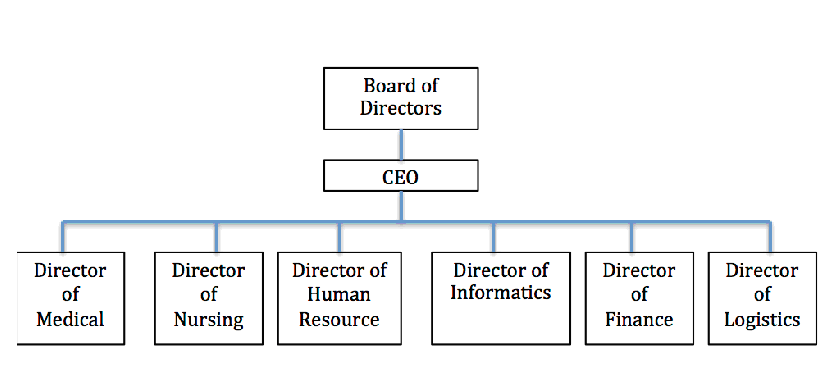
\includegraphics[width=0.9\textwidth]{organigram.eps}
  \end{center}
  \caption{Sint Jan Hospital organigram}
  \label{fig:organigram}
\end{figure}


HR department is part of top management, and is actively involved in all major decision-making.
Organization has flat hierarchy within each department.
Human resource department is relatively small with 9 -10 people.  

\section{Recruitment}

\subsection{Forecasting}

Organization has not witnessed any major expansion during recent years.
Most of the recruitments have been for replacement positions.
In case of major expansion, estimation is based mostly on government regulation and subsidy.
To give an example, in case of cleaning work government regulation plays a decisive role, which defines people to be employed for a given cleaning area.
During the forecasting period, the HR department does not employ any mathematical or statistical methods.
If the possible employment would have exceed 2 months period, selection is often made for a permanent position. 

\subsection{Recruitment}

Hospital employees various means to recruit based on the job profile and department.
Recruitment process is adapted according to department or managers needs.
The decision to start recruitment is taken together with concerned department management.
Management of the concerned department often provides the job description.
As the hospital does not generates new job positions most of the descriptions do not change. 

Job analysis for the higher management is often more difficult one, as it changes according to demand.

\subsection{Attractiveness of organization}

Being a public sector hospital they offer candidates an opportunity to serve for the society and to help people.
Job stability is other strong point of the organization. 


\subsection{Sources of Recruitment}

All vacancies are posted on the hospital web page.
And they are forwarded to the Actris or VDAB, which is a government agency to advertise vacancies.
HR department accepts CV internally from employees too.
Job advertisement on prominent newspapers is restricted to few important vacancies, as they are expensive.
External headhunters are employed for recruitment of the top management or board of directors. 

University graduate or campus recruitments are seldom practiced.
Only the nursing department hires through college recruitments.


\subsection{Recruitment Efficiency}

Efficiency of recruitment is not often measured quantitatively.
A more informal and personal measurements do exist, but they are not documented and aren’t part of organizational process.

\section{Selection}
 
\subsection{Selection Criteria}

Job description is primary input to the selection.
Fluency of local language and personality of the candidates along with technical abilities are considered as selection criterion.
Past professional experience and employee honesty with previous organizations play a role too.
Gut feeling sometimes plays a role in selection procedure.
Self-description of one’s personality in a CV is often ignored, a face to face to talk will be a major deciding factor. 

Most often age or sex doesn’t have any considerable influence.
Some job descriptions implicitly imply specific gender but they are not necessarily the requirements.
Government regulations and obligations do play some role in the selection.
The government subsidy decides on selection of handicapped people.
Government benefit to older people does play some role, but is not often a major factor to reject a candidate.
Internal candidates are evaluated with the same standard as the external.

Selection criterion for the higher management is often difficult and decided together with top management.


\section{Selection Process}

\subsection{Preliminary Selection}

Selection process often starts from HR department.
HR department prepares a shortlist of candidates with respect to academic, linguistic qualifications.
The shortlist is based on the Curriculum Vitae.
In some cases, where department managers expect more control on recruitment resume shortlisting is assisted by department managers. 

\subsection{Employment Interview}

Shortlisted candidates are invited for interview.
The number of invited candidates depends on the involvement of department managers – the more involved the targeted department is in the recruitment process; the more candidates take part in the process.
The maximum number of people interviewed is four.
Interviews follow behavioral description method i.e. Gedragsgericht interview. 

\subsection{Selection Decision}

Decision to select a candidate lies with department manager.
Director of the Human Resource does salary negotiations.
Many cases the selection process has to be restarted as salary negotiations fail to select an effective candidate.


\subsection{Probation Period}

Successful candidates need to work for a probationary period of 6 months.
This provides an opportunity for the hospital to evaluate the candidate.
The candidate can also decide if the job is as per his expectation.
The probationary period is mandatory as per the government law on employment.
At the end of probationary period a formal meeting with candidate and manager will be held.
If both the parties find no problem then candidate is considered permanent employee.


\section{Recommendation}

Sint Jan hospital is an organization fully dependent on governmental support.
The politics does not only decide on the hospitals’ budget (which is strictly correlated to the total number of employees),
but also draws the legislation, which has an imminent effect on many health care policies.
Therefore, the abilities of the Human Resources department to change its practices are strongly limited.
Nevertheless, we would like to propose a few recommendations, which should improve the recruitment processes within the hospital. 

\subsection{Human Resources and Social Media}

Firstly, we would like to point out the role the social media plays in todays’ recruitment procedures.
According to a KPMG report, 76 percent of U.S. companies used LinkedIn’s database to recruit candidates or post information about job openings.
Almost 50 percent of job seekers have done a job hunt on Facebook.
The change is inevitable as more and more young people use social media instead of more traditional form of communication.
41 percent of 2011 university graduates used social media in their job search and 61 percent of the people do not use the company’s support group first –
the social media are much more appealing for them.
The acquisition of social media into the recruitment practices seems unavoidable –
social networking is the fastest growing social media behavior online.
59 percent of global Internet users managed their online profile on a monthly basis \cite{kpmg}. 

Social Media is a powerful tool – it can help accelerate the whole recruitment process – starting with posting openings,
through pre - selection of candidates, making an offer and further monitoring after hiring.
Social Media can also facilitate integration of employees via interest groups.
Additionally, such groups can form a directory of skills and provide the HR department with a database of information about the employees. 

Another advantage of social media use is the possibility of more regular, real – time feedback.
Organizations can issue more often evaluation sessions,
get immediate insight into team’s performances sessions from internal and external partners \cite{kpmg}. 

In order to develop and effective social media strategy several important factors need to be taken into account.
The most important one is the meeting of two different generations at one company, often working together on the same projects.
While traditionalist and baby boomers prefer prefers a face-to-face encounters and telephone calls,
Generation X and Y would rather send a text and build relationships via social media.
In order to implement an efficient social media strategy a thorough research of the stakeholders’ group and impact assessment is needed.
Baby boomers are technologically savvy and do not have any problems with adapting Facebook and other social tools.
However, the process of introducing these tools has to be different for them, than for the Generation X.
It is also worth mentioning, that contrary to popular believe, the use of social media can increase productivity \cite{kpmg}.
It is worth mentioning that the Human resources departments are primarily responsible for creating organization’s social media policy. 

\subsection{Potential risks associated with social media}

One of the main risk of developing a social media policy within an organization is the struggle of successful integration it into everyday life.
The lack of success can be contributed to missing policies governing the social media usage and lack of enforcement and employee engagement.
However, the implementation of social media is inevitable.
Therefore, it is essential to keep the employee goodwill, facilitate communication among employees and avoid reputation damage. 

Social media can be associated with sets of risks – internal and external.
The internal risks include leak of privileged information,
creation of discoverable internal records concerning employment matters and introduction of sensitive information into the workplace
(politics, religion, sexual orientation).
The external risks are mainly related to the bad image of an organization
– building a negative sentiment towards an organization (by negative comments made online),
commentary in company’s financial performance, mis-representation of organization’s position on public issue and damage of reputation \cite{kpmg}.
It can be clearly seen, that social media give a lot of power to the users of a service or buyers of a good.
The organization can no longer (at least, not as easily as previously) shape the message it is sending to its consumers. 

Social media policy is a challenge.
It does not however differ from other problems businesses had to face in the past.
Moreover, many organizations already have a framework for communication – the main challenge is to redefine this framework,
so it could include the social media provisions.
In creation of a new policy all of the departments should be involved, however,
the Human Resources department could play the most important role, as it will assure the necessary balance between workplace and personal use. 

As every policy it should have a clear division of mandatory actions and consequences for not complying with the rules.
The guidelines should be easy to comprehend and to follow.
They should lie within the set of company’s values and believes.
The framework would be considered effective when it will be beneficial for building organizational knowledge and facilitating the communication flow. 

\subsection{Skill Inventory}

Skills inventory are defined by the Business dictionary as:
\emph{listing of abilities, capacities, qualifications, and career goals of the employees to identify suitable candidates for internal recruitment or promotions} \cite{BusinessDictionary}.

Skills inventory can help create a useful database of employees’ skills, talent, knowledge and attributes.
It can help reassign workers to new projects, providing the best possible combination of talents.
Accordingly, we can build a team strongly focused on particular problem or create a more holistic approach and group specialist from different disciplines.
The Human Resources department is given the freedom to combine the needed skills in most beneficial way.
It gives the company the opportunity to us its current employees and do not engage in costly and time – consuming external recruitment processes.
Geography, division or demographics can allocate the specific skills.
The strengths can be easily identified and correlated with organizational programs.
Moreover, all training programs can be deliberately target to the groups.
Skills inventory should also be closely correlated with employees’ satisfaction level.
They will be able to work on interesting projects and no person should be misplaced. 

\subsection{Outsourcing }

During recent years outsourcing has become more and more attractive for many companies, non – governmental and governmental organizations.
Some scholars consider outsourcing as the future of human resources management \cite{adler2003making}.
Adler distinguished six main factors, that companies should considered when it comes to outsourcing decisions:
\begin{enumerate}
  \item Dependency risks;
  \item Spillover risks;
  \item Trust;
  \item Relative proficiency;
  \item Strategic capabilities;
  \item Commitment versus flexibility.
\end{enumerate}
Apart from the above-mentioned risks, outsourcing also has many advantages.
One of them is the possible fluctuation of demand for human capital.
The number of employees can differ depending on the current needs of a company.
This type of employment is particularly popular at companies where numerical flexibility is particularly important.
In situations, where a company demand for employees rises, the labor force will be recruited by means of employee leasing rather then long-term contract.
The labor costs are minimal, as the temporary employees do not look for a stable, long-term job \cite{stefan}. 

The main opposing power to the outsourcing of employees consists of trade unions.
Although the temporary workers are usually not unionized and have different objectives than permanent personnel,
the increasing number of outsourced employees put pressure on labor unions.
Many European movements are currently lobbying on the EU level for better working conditions and minimum social benefits for the leased employees.
The pressure lies also on governmental regulations. 

Outsourcing techniques are mainly useful for small and medium enterprises, as it generates sales and products.
Outsourcing non-core activities can allow the company focus on their main area of expertise.
According to Toddi Gutner several questions need to be answered before taking a decision about outsourcing.

\begin{enumerate}
  \item How big is you company? Many scholars and owners of SME advise to outsource some of the activities, “when administrative processes begin slowing down the productivity of the firm” \cite{gutner}. This is an individual assessment, which should be done independently in every case. However, some employment agencies do not cooperate with companies with fewer than 10 employees. Also, it is much more efficient for big companies to have an in-house human resources department. The ideal number of employees for outsourcing to be proven efficient is between 16 and 80 people \cite{gutner}.
  \item How much does outsourcing cost? The cost of outsourcing depends on the company. Many experts estimate that the real cost varies between 2 and 11 percent of wages. In other words it would cost between \$500 and \$1,500 per employee per year \cite{gutner}. Many businesses does not estimate the costs of a human resources department – they mainly focus their attention on wages and do not take into account a total cost, which is usually hard to calculate.
  \item How much control do you want over your HR functions? Outsourcing company acts as a business partner. If the owner of the company wants a total control over all companies operations, outsourcing would not be beneficial. Businesses do loose some flexibility while outsourcing employees. Another downside of this approach is the lack of connection between employer and employee, as the latter is only dependent on the outsourcing business.
  \item What services do you need? It is important that the outsourcing company is recognizable, has some kind of official certification and has experience in the client’s industry and covers the company’s territory \cite{gutner}. It is also worth mentioning that some outsourcing companies specializes in high-tech business solutions, while other focus on more traditional business and stressed the importance of face-to-face communication. 
\end{enumerate}


\section{Conclusions}

Sint Jan hospital is in a unique position when it comes to shaping its human resources management. On the one hand it is fully dependent on the current political situation. The amount of available subsidies from the government is fluctuating every year. Moreover, any new piece of legislation, both on the national and European level, can have a serious effect on hospital’s functioning. It is also important to mention the role the healthcare system plays in a society. It can easily attack by a populist party and become a sort of bargaining card in election. This factor is especially vital during a crisis, when the society is prone to any extremist political behavior. 

The human resources department has to balance its activities between various actors and operate in constantly changing environment. This is probably why it has developed a set of rules and is not keen to change it. But in our opinion, implementing three rather easily accessible solutions can improve and facilitate running of a whole department. 

Firstly, implementation of a social media policy is essential. Social networking is an inevitable step in development of human resources management. It can facilitate the communication and cooperation between employees. The majority of recent university graduates uses websites like LinkedIn while searching for a job. If the Sint Jan hospital want to remain an attractive employer to the youth, its presence on social media is vital. Moreover, the employees themselves will use social media tools at work. Establishing clear set of rules and regulations will prevent them from developing their own, often unproductive and unwanted, behavior. 

Secondly, skills inventory should be developed. The hospital already performs an internal recruitment processes – database of all talents and skills current employees already posses, will definitely make this process more efficient and much faster. 

Thirdly, some of the current jobs should be transferred to an outsourcing company. The human resources department will be able to downsize and focus its attention on the high profile hiring. The HR department could therefore be more helpful to other departments. The size of the hospital should not be a factor, as only some of the jobs will be outsourced – for example accounting or cleaning services. 

There is a room for improvement. While working on new solutions, one cannot forget about the importance of maintaining the already existing good practices. The main goal now is to pursue new challenges and find a way to make them work with the already existing accomplishments. 

\newpage
\addcontentsline{toc}{section}{References}
\bibliography{bibliography}
\bibliographystyle{apalike}

\newpage
\appendix

\section{Interview transcript}


\question{Can you give us an overview of the organizational structure and its hierarchy.}

I’ll show you the organigram. So we have 6 big departments. Medical department, nursing department, administrative and financial department, informatics, human resources and technical and logistics department. And those are the 6 directors. Under each department you have like the different services. We have 1100 – 1200 workers here. And yeah, it’s kind of flat here the hierarchy, pretty flat. To give you an example, the most important department. Well maybe not that well put, but the department most people are in is the nursery department and you have the care-coordinators, it’s like the middle management and then you have the head nurse. That’s pretty much the hierarchy. So if the nurse wants to go up on the scale first they would be head of the department and then care-coordinator and then you are already at the director level. It’s pretty flat on all the levels in all the departments.  

\question{I presume that you are not in charge of the HR department when they hire the doctors.}

No. Doctors are independent and they are…

\question{… drawn in by the medical board.}

Yeah. And as well for the nurses. They are brought in by the nursery department. So what we do here on the HR department, we do different things for all the hospital, less for the doctors. But we do the recruitment for the other departments. 

\question{Can you give us some idea of the HR department? How is it organized? What is the size?}

It’s pretty small. (scrolls on the PC) This is our department. So we have the director, Chantal bony (?), and you have two people who actually do other things like translation and we have a language coach. The real department is like 9 persons. One of them, we’re going to start with myself, I do the selection and recruitment and different HR things on different levels. Two people are the secretaries who do the administration for the other people. And then you have 6 people who are in charge of the cell contracts and the cell payments. Each cell has three persons. So that is how we are organized: Contracts, pay and then more HR related processes, more soft HR.  

\question{And is there a house style of doing HR in Sint-Jan Hospitaal?}

That’s a really difficult question. When you have an overview of different companies you might see differences but when you are in a company it is really difficult to see what kind of thing you do. 

\question{I think when we advance in the questionnaire there will be a style that becomes apparent. I think the question is are you aware of the fact that you have a certain style or a certain strategic approach to HR?}

And what could be a possible style for instance? Is it determined? 

\question{There are different styles but it’s more like has there ever been a brainstorm session about how are we going to approach the HR department in Sint-Jan. Or is it something that has grown throughout the years?}

It’s organic yes. What is important is that the HR director is part of the management team. Which is not the case in all companies. Sometimes it depends on like financial or administration department but here it’s like a real manager in itself. So we give a lot of importance to HR. Maybe not in person but in idea, the HR manager is there where all the important decisions are made. So that’s maybe one little part. She’s there since 30 or 25 years and she first wasn’t part of the management team but she became so it grew very organically. This is the social profit sector so we take in account that people are important for us. We have some constraints and things to obtain financially but it is not our goal. Our goal is to help the people.  

\question{How many beds does this hospital have?}

473. Which is like middle. 

\question{Yeah, because my dad works in a hospital and 473 is not a lot to have a HR department. I think the HR department isn’t that small for a hospital that has this many beds.}

What is important to know is that we do all the payment ourselves. We don’t have a social secretariat (who takes care of the payroll). So that might explain the size. And we try to care for the people who work here within the constraints of the economy and the financial … but maybe that’s not a good answer to your question. 

\question{How do you plan future HR requirements?}

Like how do we know how many people we have to hire? 

\question{Yes.}

Well, it was a funny question for us because we don’t work like that at all. It’s not like real planning. In the daily work someone falls ill or resigns so we look for someone new if the circumstances are always the same. When the circumstances change we do something else. 

\question{So you have a fixed number of employees that you know we need this many to have a efficient working hospital.}

Yes, and a lot of those numbers is based on what is legally allowed for hospitals to have or what is subsidized. So a lot depends on that. When things change or when there is a department where there is need for someone with specific qualifications we might hire him/her when the financial situation allows it. But like the list of theoretical tools we don’t use them at all. 

\question{The thing is we come from the business economic side of things so we thought it would be interesting to apply the business side of HR management to the health care sector.}

Well maybe on a higher level. For instance for a specific amount of square meters you can hire x number of cleaners. And that is legally well defined. Well maybe in the past it has been calculated how many employees were needed but now it’s pretty fixed. And it changes when it’s really necessary. 

\question{Have there been changes in the number of employees these past years?}

Definitely. It has risen because we had a fusion as well with another hospital so things have changed a lot. But then we see that some functions have to be created because they become more and more important. For instance the informatics  department, it was necessary to have more people but then we see what is needed and what is financially possible and then we go for it. 

\question{Do you maintain a skills inventory of employees?}

More informal. Like  when somebody wants to switch to another function we try to think about it when that function becomes available. But for the training and development programs we don’t have something like that. In another company I saw that every employee had a page on the internet with things he liked and things he did in his free time so when somebody wanted to make a video they could call maybe the cleaner who could… But no, we don’t have that. A lot of people work here for a long time. Definitely the chefs, the heads of department and they know what goes on in their unit and they know who wants what so they try to find ways to help people when they want to do another task or another job. 

\question{So in that respect you actually pay a lot of attention to interpersonal relationships.}

 We try as much as possible. 

\question{ When I apply for a job and am let down, more often than not I get told that my CV is being kept. Do you do that?}

(Shows the boxes with resumes) 

\question{That answers the question.}

This is just the paper that arrives. We keep all the CV’s for a year. And then in theory, we have a recruitment base where we keep all the people in. But then in reality, we get so many cv’s that it’s impossible to go look for one who applied in January when we are already in November. But for some jobs we don’t have that much candidates and then we go and search the recruitment base. We do that, but it depends on the function. 

\question{So what you’re saying is when there are a lot of applicants you prefer someone who has just applied over someone who applied earlier.}

Yes, because you know about that one that he is free. Practically when I need someone for the cleaning department I have a colleague who drops all the CV’s, then I take the first twenty, invite four and that’s how it goes. And then people call and call and call and then sometimes I say come on. “I don’t want to hear you anymore. Come on, I’ll see you and I’ll decide whether or not it is possible.”

\question{You kind of already answered this but is recruitment based on the individual need of business units (the different departments) or is it more from the top management.}

It depends. If someone resigns, we need someone to fill the place. Then I talk to the head of the department and we go on. But when the situation changes or the HR director says “hmm, I’m not really sure if we need someone there” then it’s the top that decides. But it really is an interaction between the two. But on the more daily things we just go on and hire. 

\question{And I presume higher functions are always decided by the board, etc.}

Yes. Also about the job content. For a lot of jobs it’s very clear what the person has to do but at director level it sometimes changes or people get other responsibilities. Then it’s often more complicated. It depends on the personality of the director as well, what he takes, what he does in his job and what not. And it’s organically as well. Some things are like that and will always be like that.
RECRUITMENT

\question{Could you give us an overview of the recruitment process?}

It depends. In here things always go like they are best. It depends on every department. And mostly on what the manager wants. Very theoretically, we have to look for someone. I go and see the manager to see what he or she wants. I make a job offering that appears through different channels. And then I get the CV’s and mostly I do a first selection. For instance, the basics, when we look for a social assistant, he or she has to have the diploma. He or she has to speak Dutch and French. If that is not the case, I don’t even transfer the CV. When I transfer the CV’s, the chef says “hm, sounds interesting” and then I either see 7-8 people and send the best 3-4 to the manager or we see people together. So we have 2 to 3 job interviews, depending on the level. Some managers want to have a good grip on what happens and they want to see all the CV’s. Sometimes they want to see the CV’s first and then they send me one person they really want to hire. But then the problem can be that that one person is not compatible on salary level. It’s more interesting that I see some people after seeing the CV’s and then I already make a selection. Because sometimes there are people that seem okay on CV but in reality… yeah. So it’s a waste of time that the manager has to accord time to that person. I’m there to make a first selection and that’s mostly the way how it goes. Sometimes there are managers that say “send me one person and if I like him I’ll hire him.” Then I do the selection until the end. 

\question{After the person has been selected and sent to the manager, do they come back again for a follow-up interview or does the person just start working the next day?}

Once I’ve had an interview I don’t have another interview anymore. If there is some question concerning salary I look to the HR director. He or she does the negotiations. Mostly the wages are fixed because we work with scales and then it’s just a question about how much seniority this person has. Mostly the salary is fixed and we say “This is our proposal, take it or leave it.” It also depends on the function. If it’s someone really good for a difficult complex function we have some maneuverability but this is not always. 

\question{And there are no scales that allow the financial needs of these highly qualified people to be met?}

Yes, there are scales for every function. From a certain level these scales are linked to the market. For some functions this is a bit problematic. For instance the informatics department, sometimes we have to acknowledge more seniority because otherwise it would not be competitive compared to the rest of the market. 

\question{This is allowed?}

It’s a choice that has to be made. 

\question{Isn’t such a thing regulated? For instance when a person who is 30 years old has 15 years seniority?}

We decide for ourselves how much seniority we give. It has to be financially feasible and it also has to be fair towards the rest of the employees. That somebody who asked a lot gets the same salary who has already been working here for 5 years. It’s always a balance between being correct and attracting the right people. We have the advantage that we can offer stability. And this attracts a certain type of person. There is sometimes a bit of a misunderstanding. Sometimes people think the social sector is a bit underpaid but this is not necessarily the case. We are not the best paying sector if you compare us to the chemical sector. But those are different things. We have other advantages. 

\question{Is this because the people require less skill than in other sectors? Or different reasons?}

It’s an image mostly. But especially for starters the social sector isn’t that bad at all. Like nurses, bachelor degree, are pretty well paid. Also because they have uncomfortable hours. Vacature sometimes makes comparisons and it’s not that bad at all, mostly for starters. But since everything is well defined, 1 year it’s this, 5 years it’s that, sometimes the leaps are smaller. 

\question{Do you prefer internal or external recruitment?}

It depends on the function. We mostly start with internal candidates. But for a lot of functions we don’t have that. We don’t have a pharmacy assistant in another department that wants to do pharmacy. But sometimes for different tasks in the same service there is an internal candidate. Then we have friends and family a lot and it’s pretty disappointing sometimes that I don’t want to hire a husband or wife or son or daughter. They are not always the best person for the function. People always tend to think that their spouse is the best person for the job but I’m not always convinced. 

\question{Why is that, that you don’t want family members to join?}

It’s not that I don’t want to. But sometimes I get a father and he says “My son is such a good guy” but when I look at the CV it’s like “I’m sorry but I have better.” My task is to choose the right person. 
So we have pages with vacancies who get seen by visitors. And externally we always use posters on the intranet and internet it’s our own page. We are also obliged to put it on Actiris, which is like the Brussels VDAB. We mostly put it on VDAB as well. And for the social job openings we put it on guide sociale, which is pretty well known for social assistants, secretaries, ... And then, but that depends on the level of recruitment, we go in press, vacatures, jobat. But we really try to restrict it because it costs an enormous amount of money. For a small advertisement its 4000 euro, nothing fancy. But sometimes we have to do it, otherwise we don’t reach the people we want to reach. Sometimes we do headhunting, like an external recruitment office that looks for someone. 

\question{Like interims?}

We do work with interims but mostly not to test people. We do hire people for a very specific amount of days. When it’s longer than 1-2 months we try to hire ourselves. Because you also pay the interim offices. 

\question{And those external recruitment offices are like assessment companies?}

Yes, for instance. And then they do the whole recruitment process. 

\question{So sometimes you outsource the recruitment process?}

Yes. And that’s like 2 or 3 jobs a year. And really only for board level jobs. 

\question{And do you prefer to hire someone who already works in the hospital or someone from outside?}

It depends. If it’s a good employee I prefer him/her because that person has experience working in this hospital. But if it’s not the right person for the job then no. And also when that person switches jobs I have to find someone else for the position he or she just left. So for me it’s the same work. 

\question{Do you have any university graduate programs?}

No. 


\question{Do you have people to recruit new graduates.}

No. Well sometimes the nursing department goes to job fairs. But for me, the persons that I have to find are so varied. KPMG or Deloitte go to a job fair because they have to find 20 accountants. I have to find one accountant and one pharmacist and two cleaning ladies and five kitchen helpers. 

\question{Do you use new social media like facebook and twitter to advert vacancies?}

No. But I know I’m going to have to. But I don’t like it at all. Myself, I’m not on facebook, I don’t see the use. Well, I see the use but I’m not an early adopter. I will do it if I really have to. And I know that we have to be active on it but I’m not interested in it at all. 

\question{So it’s more for personal reasons?}

Yes. It’s just me. 

\question{And why do you think you have to?}

Because the young people we hire, for instance the nurses here, start at 21. We have a lot of young incoming personnel and that’s how they grew up. How they work.  So we have to jump on the band wagon and everybody keeps telling us we have to. 

\question{In my experience it’s normal for big companies, like coca-cola, to be on facebook, but it would be weird to see a hospital on facebook.}

There is like an ambassador, Lon Holser, that is imploring companies of the social sector to be more active on social media. So it is a movement that’s coming up and hospitals are not the first to jump on that. Twitter will be more difficult I feel, but linkedin, there has to be a presence. I had some trouble using linkedin some time ago and the result is nothing happened. But I’m working on it. What is difficult is that it is not the most urgent matter. What is urgent is that they need someone tomorrow at the reception. So it’s always something that comes after all the rest. 

\question{In terms of recruitment it is the most direct way of reaching people I feel. You’re in your office, you type some lines, press enter and people see it immediately. And probably the most cost-efficient one as well.}

Yes, and also the key search words in Google is something we have to work on as well. 

\question{Do you communicate your company values to the public?}

No, not really. The head of the nursing department does go to job fairs and he goes to schools as well. So he has this way of explaining what we stand for and why we are important. But for me it’s more difficult because we look for different profiles and people. We could do that on our website for instance, but only when you have to go and look for it. We don’t want to force it on people. We also kind of expect people to know when they enter a hospital what we find important. But maybe it’s too implicit. 

\question{This may be a controversial question. But during the recruitment process do you give preference to certain demographic criteria like age, sex.}

Not in theory, not at all. But for some jobs. When we need a cleaning lady for the changing room, we’re going to put a woman there, not a man. Now I’m looking for someone to do the reception in the morgue and it’s kind of a physical job so I maybe looking implicitly for a man. But if there is a woman who shows she can do the job, I have no problem with that. Age is another thing. We have a lot of people over 45 because there is this plan that companies have these days concerning the employment of 45 plussers, and we score pretty well on that. But what is a bit annoying is the fact that they have a lot more holidays. So a nurse who is 55 has 36 extra days of holiday. So that’s 36 on top of the usual 20-24 we have. 36 Just because she works in a hospital and is a nurse. So that means you have this person 4/5th of the time instead of full time and you pay the same. We have a shortage of nurses so we hire who ever we can get but for other jobs, sometimes it’s a bit difficult. When a manager has the choice between someone who is 35 and 58 and they both have the same qualities but one works full time and the other only 4 days for the same pay… then the choice is sometimes a bit difficult (she meant easy). But for us, age and what age brings with it is part of the person itself. The language skills, the skills, the motivation. Each one is part of this person’s criteria which we take in account. 

\question{I read in an article that companies are more likely to hire younger people because they are more motivated, cost less, are more willing to work harder. Do you take this into account when hiring?}

No, not at all. We look more to the personality. You have very energetic 45 plussers and youngsters who are not energetic at all. 

\question{This has been answered briefly already but do you sometimes outsource parts of the recruitment process.}

Yes, for the higher level jobs. And sometimes, for instance when we want to hire a head nurse, we outsource the assessment, but only the assessment. 

\question{Is the government restricting the way you do HR in any way?}

No, we are free to do what we want. But for some subsidies there are certain conditions like age of people we hire, or length of previous unemployment. But those are not things I look for when I do the recruitment. It’s more my colleagues who are excited afterwards when I’ve hired an unemployed. But I’m looking for the best candidate and sometimes there are things that work out nicely, subsidy wise. 

\question{What do you think is your best value?}

What attracts people is ‘to want to work for people’. To be in a company whose main drive is to help people. And stability. 

\question{Do you employ some way of measuring recruitment efficiency?}

No. Implicitly I try to learn and to see. 

\question{The fact that you have a lot of long-term work relationships implies that you are doing a good job.}

Yes. But when you are working with people there are always things that arrive on the surface. And it’s sometimes disappointing to see that they sell themselves very good and then when they are employed it seems to be different. We work with people, so we can’t predict how they will turn out. We see people for 30 to 45 minutes and then you have to decide whether they are good or not. And we are all humans so sometimes you’re wrong, sometimes you’re right. What is difficult is that the ones you refuse, you’ll never know if they would have been a good employee or not. The ones you hire you can always say this was good, this was not. But you never see the other way around so it’s difficult to adjust your way of working because you only have a very small part of the information. 

\question{Do you follow the textbook standards in recruiting or do you adapt to your own liking?}

You always adapt. What I try to do when I do the interview is to focus on things in the past and not ask ‘How would you do this or that?’. More ‘Can you tell me about a situation where you showed this or that?’, to talk about things that happened to find out how people are like. I try to listen a lot and don’t tell that much. I follow the book ‘Gedragsgericht interview’ (Behavior wise interviewing).

\question{Do you have a probation period after hiring someone?}

Yes. Always. Mostly, when we give a contract of an undetermined length it is six months. 

\question{And why is that?}

To see if things work out. And for the person as well to see if the job suits him. But it’s legal as well. 

\question{And what happens after these 6 months?}

Then we have an evaluation. Well, it’s not an evaluation. We call it more of a conversation between chef and employee to see what goes good and what could be improved. If things go really bad then it’s clear, we stop the contract. But sometimes there is an adaptation necessary and after 5 months or so we have a real evaluation to see if we go on with this person or not. 

\question{Do you know about the Hay’s method of compensation?}

Has that to do with function classification?

\question{Yes.}

No, we have our own scales that we follow. And they are conform to the hospital sector. That’s PC 330 that we follow. (PC= Paritair Comité but that is really hard to translate to English) 

\question{Do you give more attention to education, languages, etc or more to the person’s personal traits, extracurricular activities, etc. ?}

What I find very important is the languages. And I always look for stability. When I see a CV with a lot of different things I’m a bit more hesitant. Because that is what we need here. People who are stable and are able to invest in something. People that have a certain way of… Difficult to say. 

\question{I think it’s a way of life that transcends the workplace but is also being a stable person as a whole.}

Yes. There are people who change every 6 months or every year. There are people in a career of 20 years that have done 20 different jobs. Then I’m like does he know what he wants? Are there problems everywhere? 

\question{Maybe it’s just a dynamic person?}

Maybe. But it’s not our way of working to train someone, then have him/her for 6 months after which we have to hire another person. 

\question{So you pay a lot of attention to specialization.}

If a person enters a company and he has experience in different departments, I don’t mind at all. But it’s a certain way of engagement to something. More than really the contents of a job. And then it really depends on the function. 

\question{Does your gut feeling play a role in recruitment decisions?}

Yes. Face to face feeling will be the most important. Combined with the technical skills that the management checks. Personality is very important. Lots of things are trainable but personality is something you have, or are stuck with. 

\question{Do people put personal things on their resume? Like I’m a driven person, or I do sports, etc?}

Yes. But I don’t tend to read that. 

\question{Thank you for this interview!}


\end{document}
